\documentclass[12pt,oneside]{book}

%%%%%%%%%%%%%%%%%%%%%%%%%%%%%%%%%%%%%%%%%%%%%%%%%%%%%%%%%%%%%%%%%%%%%%%%%%%%%%%%%%%%%%%%%%%%%%%%%%%
%                                                                                                 %
% The mathematical style of these documents follows                                               %
%                                                                                                 %
% A. Thompson and B.N. Taylor. The NIST Guide for the Use of the International System of Units.   %
%    NIST Special Publication 881, 2008.                                                          %
%                                                                                                 %
% http://www.nist.gov/pml/pubs/sp811/index.cfm                                                    %
%                                                                                                 %
%%%%%%%%%%%%%%%%%%%%%%%%%%%%%%%%%%%%%%%%%%%%%%%%%%%%%%%%%%%%%%%%%%%%%%%%%%%%%%%%%%%%%%%%%%%%%%%%%%%

\input{../../../../Bibliography/commoncommands}

% Load packages
\usepackage{graphicx}

% Rename chapter headings
\renewcommand{\chaptername}{Section}
\renewcommand{\bibname}{References}

% Math shortcuts
\renewcommand{\sb}[1]{_\mathrm{#1}}
\renewcommand{\C}{\mbox{C}}
\renewcommand{\H}{\mbox{H}}
\renewcommand{\O}{\mbox{O}}
\newcommand{\N}{\mbox{N}}

% Center all figures
\makeatletter
\g@addto@macro\@floatboxreset\centering
\makeatother

\begin{document}

\bibliographystyle{unsrt}
\pagestyle{empty}

\begin{minipage}[t][9in][s]{6.25in}

\headerB{
Impact of Hose Streams on Air Flows inside a Structure
}

\headerC{
\flushright{
Daniel Madrzykowski \\
Craig G. Weinschenk \\
Kristopher J. Overholt \\
{\em Fire Research Division \\
Engineering Laboratory \\
Gaithersburg, Maryland, USA} \\ }
}

\flushright{\today \\
}

\vfill

\flushright{
\includegraphics[width=2.in]{../../../../Bibliography/nistident_flright_vec} \\[.3in]
}

\titlesigs

\end{minipage}

\newpage

\frontmatter

\pagestyle{plain}
\pagenumbering{roman}

\cleardoublepage
\phantomsection
\addcontentsline{toc}{chapter}{Contents}
\tableofcontents

\cleardoublepage
\phantomsection
\addcontentsline{toc}{chapter}{List of Figures}
\listoffigures

\cleardoublepage
\phantomsection
\addcontentsline{toc}{chapter}{List of Tables}
\listoftables

\chapter{List of Acronyms}

\begin{tabbing}
\hspace{1.5in} \= \\
FDS \> Fire Dynamics Simulator \\
HGL \> Hot Gas Layer \\
HRR \> Heat Release Rate \\
HRRPUA \> Heat Release Rate per Unit Area \\
NIST \> National Institute of Standards and Technology \\
\end{tabbing}

\mainmatter

\chapter{Introduction}
\label{chap:Introduction}
NIST has conducted a significant amount of research examining how ventilation affects the growth and spread of fire within structures and how the air flow to the fire may be controlled to limit or delay the growth of the fire. The studies have resulted in guidance to the fire service regarding ventilation tactics. However, ventilation tactics alone will not result in the complete extinguishment of the fire; fire suppression with hose streams are needed.

Fire suppression tactics using hose streams also affect the ventilation in a structure and can impact the movement of smoke and heat through a structure as vents are made to advance the line or if ventilation inducing hand line tactics are in practice. This research addressing the coordination of suppression tactics and the impact on ventilation is needed to complete recommendations on fire control tactics to appropriate standards, education, and training documents.

This report is concerned with examining the impact of hose stream selection and the pattern in which the stream is applied on the ventilation inside a structure with various flow path configurations. Two types of experiments were conducted in order to examine the impact. First, cold flow tests were performed. These tests involved using a 0.46 m (18 in) diameter positive pressure ventilation (PPV) fan to move air through a structure with various flow path configurations. The second type of experiment involved flowing water using various stream and application patterns into a structure with flow path configurations similar to the cold flow test configurations. Air velocities measured during the hose flow experiments were compared to the velocities measured during the cold flow tests to determine the impact of hose stream and application pattern combinations on ventilation throughout the structure relative to the impact of using a 0.46 m (18 in) diameter PPV fan to move air throughout the structure. 

Three types of hose streams were each applied in four different fashions during each set of hose flow experiments. The three types of hose stream patterns studied were straight stream, narrow fog stream, and wide fog stream. Water was flowed into the structure by having the hose in a static, fixed position, moving the hose line left-to-right across the room in a sweeping motion, and rotating the hose line in both the clockwise and counterclockwise directions.

\section{Background}
\label{sec:Background}


\chapter{Experimental Setup}
\label{chap:Experimental_Setup}

\section{Experimental Structure}
\label{sec:Experimental_Structure}

\subsection{Construction}
\label{sec:Construction}
Two structures, shown in Fig.~\ref{fig:struct_pics}, were constructed for the experiments. Each structure contained a ground level floor composed of walls surrounded by concrete blocks. The West Structure contained a second level.

\begin{figure}[!ht]
\includegraphics[width=6in]{../../Figures/east_structure}
\\~\\
\includegraphics[width=6in]{../../Figures/west_structure}
\caption[East and West Test Structures]{East (top) and West (bottom) Test Structures}
\label{fig:struct_pics}
\end{figure}

\clearpage

\begin{figure}[!ht]
\includegraphics[trim=0cm 0cm 0.75cm 4.5cm, clip=true, width=6in]{../../Drawings/PDFs/Without_Instrumentation/West_Structure_1st_Floor_Metric_Simple}
\\
\includegraphics[trim=0cm 0cm 0.75cm 5.0cm, clip=true, width=6in]{../../Drawings/PDFs/Without_Instrumentation/West_Structure_2nd_Floor_Metric_Simple}
\caption[West Structure first and second floor layouts]{West Structure first floor (top) and second floor (bottom) layouts. All dimensions are in meters.}
\label{fig:west_general_plan}
\end{figure}

\clearpage

\section{Instrumentation}
\label{sec:Instrumentation}
Schematic plan overviews of the instrumentation in the East and West Structures are shown in Fig.~\ref{fig:east_instrumentation} and Fig.~\ref{fig:west_instrumentation}, respectively. There is a discussion of uncertainties for each measurement below in Section~\ref{sec:Uncertainty}. Gas velocity was measured at various doorways using differential pressure transducers connected to bi-directional velocity probes~\cite{McCaffrey:Combustion_and_Flame}. Each set of BDPs contained 8 probes located at distances of 0.08 m, 0.34 m, 0.61 m, 0.88 m, 1.15 m, 1.42 m, 1.68 m, and 1.95 m below the soffit of the corresponding doorway. Fig.~\ref{fig:BDPs} shows a picture of two sets of BDPs, A5 and A6, located at each double door on the first floor of the West Structure. A single thermocouple was attached to each bi-directional probe. The thermocouples used with the bi-directional probes are exposed-bead, Chromel-Alumel (type K) with a 1.0 mm (0.04 in) diameter. Starting with the exposed bead, the thermocouple wire was sheathed in a 3.2 mm (0.13 in) diameter Inconel shield, 0.76 m (2.5 ft) in length.

%\begin{figure}[!ht]
%\includegraphics[trim=0cm 0cm 0.75cm 4.5cm, clip=true, width=6in]{../../Drawings/PDFs/With_Instrumentation/East_Test_Structure_Devices_Hose_Test}
%\caption[Location of Instrumentation in East Structure]{Location of Instrumentation in East Structure}
%\label{fig:east_instrumentation}
%\end{figure}

\begin{figure}[!ht]
\includegraphics[trim=0cm 0cm 0.75cm 4.5cm, clip=true, width=6in]{../../Drawings/PDFs/With_Instrumentation/West_Test_Structure_Devices_Hose_Test_1st_Floor}
\\
\includegraphics[trim=0cm 0cm 0.75cm 5.0cm, clip=true, width=6in]{../../Drawings/PDFs/With_Instrumentation/West_Test_Structure_Devices_Hose_Test_2nd_Floor}
\caption[Location of Instrumentation in West Structure]{Location of Instrumentation in West Structure}
\label{fig:west_instrumentation}
\end{figure}

\begin{figure}[!ht]
\includegraphics[width=6in]{../../Figures/BDPs}
\caption[Two sets of BDPs in Doorway]{Two sets of BDPs, A5 and A6, in each doorway of the double doors on the first floor of the West Structure}
\label{fig:BDPs}
\end{figure}

\section{Uncertainty}
\label{sec:Uncertainty}
There are different components of uncertainty in the length, differential pressure, and gas velocity reported here. Uncertainties are grouped into two categories according to the method used to estimate them. Type A uncertainties are those which are evaluated by statistical methods, and Type B are those which are evaluated by other means ~\cite{Taylor&Kuyatt:1994}. Type B analysis of systematic uncertainties involves estimating the upper (+a) and lower (-a) limits for the quantity in question such that the probability that the value would be in the interval ($\pm$a) is essentially 100\%. After estimating uncertainties by either Type A or B analysis, the uncertainties are combined in quadrature to yield the combined standard uncertainty. Then, the combined standard uncertainty is multiplied by a coverage factor of two, which results in the expanded uncertainty with a 95\% confidence interval (2$\sigma$). For some of these components, such as the zero and calibration elements, uncertainties are derived from referenced instrument specifications. For other components, referenced research results and past experience with the instruments provided input in the uncertainty determination. 

Each length measurement was taken carefully. Length measurements such as the room dimensions,
instrumentation array locations, and fire apparatus (for example nozzle, sprinkler, or fan) placement were made with a hand held laser measurement device which is has an accuracy of $\pm6.0$ mm (0.24 in) over a range of 0.61 m (2.00 ft) to 15.3 m (50.0 ft)~\cite{Stanley}. However, conditions affecting the measurement, such as levelness of the device, yield an
estimated uncertainty of $\pm$0.5\% for measurements in the 2.0 m (6.6 ft) to 10.0 m (32.8 ft) range. Steel measuring tapes with a resolution of $\pm$0.5 mm were used to locate individual sensors within a measurement array and to measure and position the furniture. The steel measuring tapes were manufactured in compliance with NIST Manual 44, which specifies a tolerance of $\pm1.6$ mm (0.06 in) for 9.1 m (30 ft) tapes and $\pm6.4$ mm (0.25 in) for 30.5 m (100 ft) tapes \cite{NIST_Manual_44}. Some issues, such as "soft" edges on the upholstered furniture, result in an estimated total expanded uncertainty of $\pm$1.0\%. 

Bi-directional probes and single thermocouples were used to measure the velocity. The bi-directional probes used similar pressure transducers as those used for the differential pressure measurements discussed above. Bare-bead Type K thermocouple are co-located with the probe. A gas velocity measurement study, examining the doorway flow of pre-flashover compartment fires, yielded expanded uncertainty measurements ranging from $\pm0.14$ to $\pm0.22$ for bi-directional probes of similar design \cite{Bryant:FSJ2009}. The total expanded uncertainty for gas velocity in these experiments estimated to be $\pm18$\%.   

Water flowrate was measured with a pressure and flow meter combination shown in Fig. \ref{fig:flow_meter}. The meter consists of a section of 6.35 cm (2.5 inch) cast aluminum pipe with a 0–4.1 MPa (0-600 psi) pressure transducer and a paddlewheel type flow sensor with a range of 0 to 4800 lpm (1250 gpm). The pressure transducer and paddlewheel both connect to the battery operated control box where the pressure transducer voltage is converted to a pressure and the paddlewheel pulse count is converted to a volumetric flow rate. The manufacturer reports a $\pm5$\% calibration expanded uncertainty for the flow sensor and $\pm3$\%  for the pressure sensor \cite{Akron}. The pressure transducer was calibrated with a known analog pressure gauge. The flow meter was calibrated by capturing water over time and measuring that mass of water to determine the flowrate. The total expanded uncertainty was estimated at $\pm10$\%. 

%\begin{figure}[!ht]
%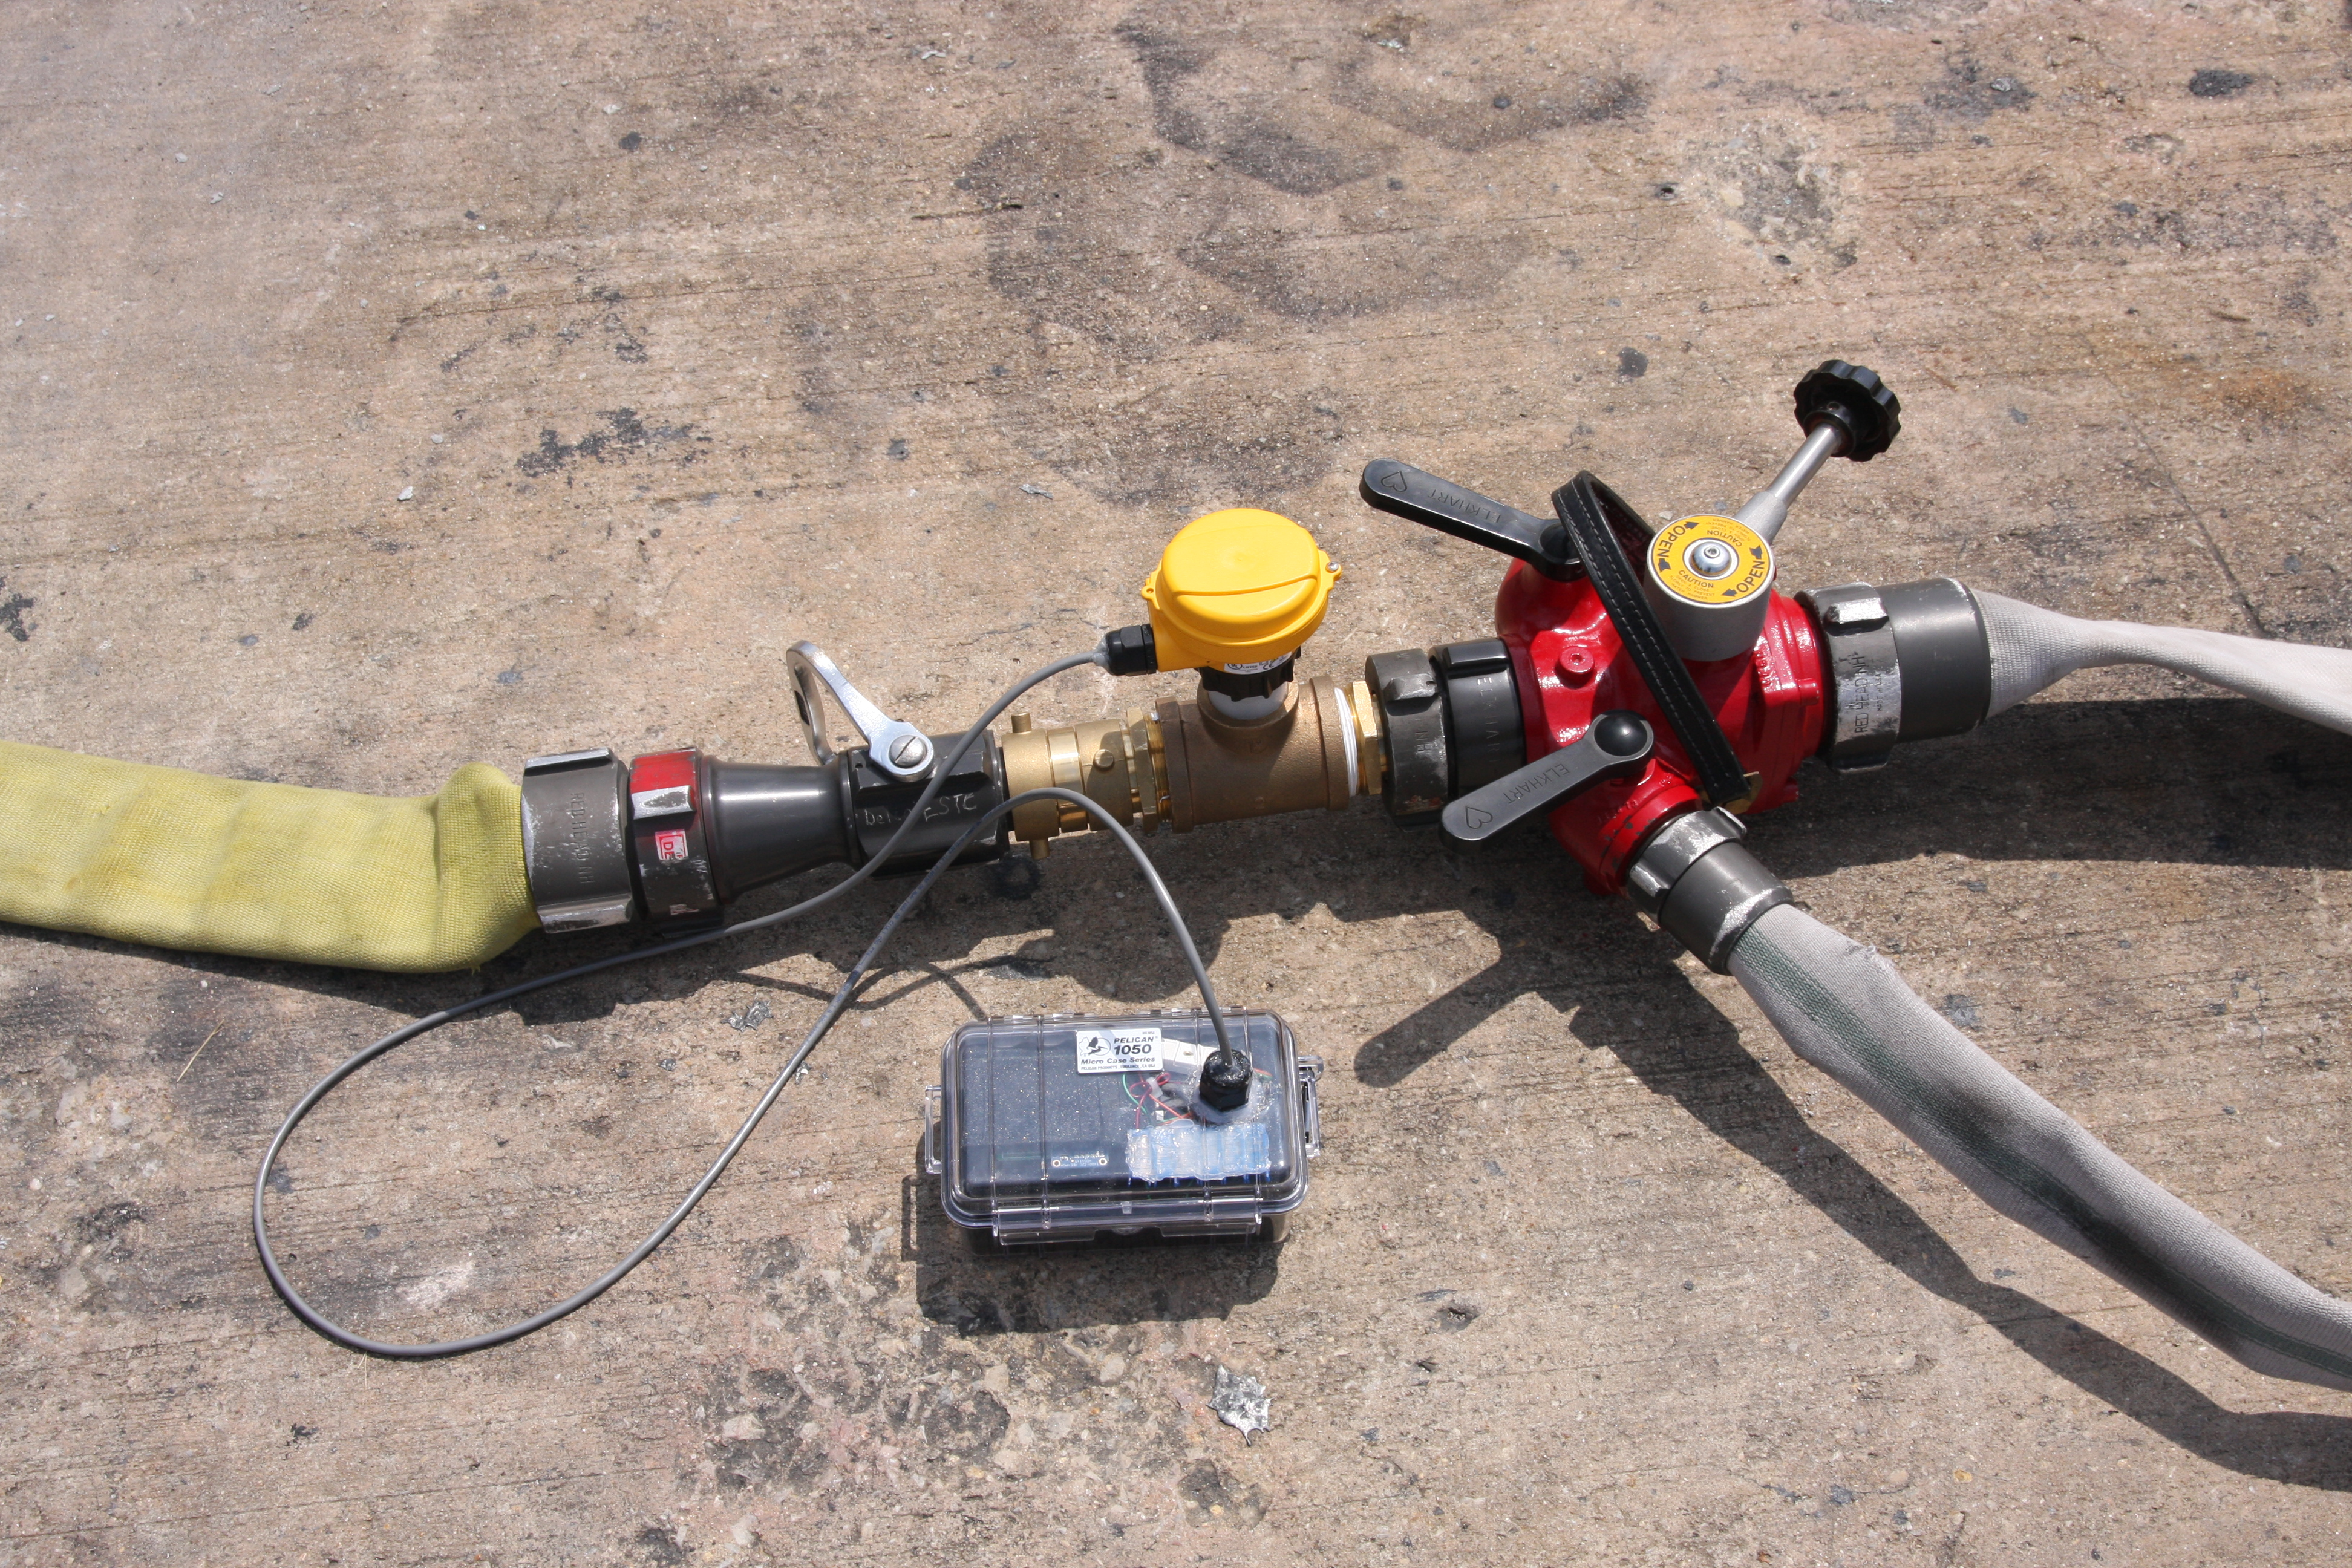
\includegraphics[width=6in]{../../Figures/flow_meter}
%\caption[Picture of Flowrate Meter]{Pressure and flow meter combination used to measure water flowrate}
%\label{fig:flow_meter}
%\end{figure}

In the following sections, the measurements will be presented in graphic and tabular form. In the graphs, an error bar will represent the estimated uncertainty of the measurement. In the tables, the uncertainty will be included in the table of as part of the caption.

\section{Experimental Procedure}
\label{sec:Experimental_Procedure}

\subsection{Cold Flow Experimental Procedure}
\label{sec:Cold_Flow_Procedure}

\subsection{Water Flow Experimental Procedure}
\label{sec:Water_Flow_Procedure}
A total of four sets of experiments were conducted to observe the impact of using different hose streams and application patterns on the ventilation in the West Structure.

Two sets of experiments involving application patterns, Tests 18 and 19, were conducted. The two sets varied in that the first floor south side door was open for Test 18 (Fig.~\ref{fig:test_18_plan}) and closed for Test 19 (Fig.~\ref{fig:test_19_plan}).

Tests 18 and 19 followed identical procedures that involved flowing water into the West Structure through the first floor, south side double doors using a 1.75 in. hose with a combination nozzle. The nozzle was used to produce three types of hose streams: a straight stream, a narrow fog stream, and a wide fog stream. Tests 18 and 19 involved three sets of experiments, one for each type of hose stream. For each set of experiments, four different application patterns were tested. First, water was applied while the hose was in a fixed position. Next, the hoseline was moved from side-to-side across the open room, creating a sweeping application pattern. Finally, the hoseline was rotated in both the clockwise and counterclockwise directions, creating clockwise and counterclockwise application patterns. 

To begin each set of experiments, the combination nozzle was adjusted to produce the desired hose stream pattern. Once the nozzle was adjusted, water was applied while the hoseline was in the fixed position. After 60 seconds of water flow, the stairwell door was opened. 60 seconds after the stairwell door was opened, the north side, west double door on the second floor was opened, and water continued to flow for 60 more seconds. Then, the hoseline and two doors were closed, and the procedure was repeated for the sweeping, clockwise, and counterclockwise application patterns.

\begin{figure}[!ht]
\includegraphics[trim=0cm 0cm 0.75cm 4.5cm, clip=true, width=6in]{../../Drawings/PDFs/Without_Instrumentation/West_Structure_Hose_Test_18_1st_Floor}
\\
\includegraphics[trim=0cm 0cm 0.75cm 5cm, clip=true, width=6in]{../../Drawings/PDFs/Without_Instrumentation/West_Structure_Hose_Test_18_2nd_Floor}
\caption[West Structure first and second floor layouts for Test 18]{West Structure first floor (top) and second floor (bottom) layouts for Test 18. Both double doors and the south side door were open on the first floor for the duration of the test. On the second floor, the stairwell door and north side, west double door were opened and closed during the experiments, while the north side, east double door and south side door were in the closed position throughout the entire test.}
\label{fig:test_18_plan}
\end{figure}

\begin{figure}[!ht]
\includegraphics[trim=0cm 0cm 0.75cm 4.5cm, clip=true, width=6in]{../../Drawings/PDFs/Without_Instrumentation/West_Structure_Hose_Test_19_1st_Floor}
\\
\includegraphics[trim=0cm 0cm 0.75cm 5cm, clip=true, width=6in]{../../Drawings/PDFs/Without_Instrumentation/West_Structure_Hose_Test_19_2nd_Floor}
\caption[West Structure first and second floor layouts for Test 19]{West Structure first floor (top) and second floor (bottom) layouts for Test 19. Both double doors were open and the south side door was closed on the first floor for the duration of the test. On the second floor, the stairwell door and north side, west double door were opened and closed during the experiments, while the north side, east double door and south side door were in the closed position throughout the entire test.}
\label{fig:test_19_plan}
\end{figure}

\begin{figure}[!ht]
\includegraphics[width=6in]{../../Figures/Test_18}
\caption[North Side of West Structure during Test 18]{North side of West Structure during Test 18. A straight stream pattern is being applied, and the flow path is fully established with the stairway door and the north side, west double door both opened.}
\label{fig:test_18_pic}
\end{figure}

\clearpage

\chapter{Results}
\label{chap:Results}

\section{Cold Flow Test Results}
\label{sec:Cold_Flow_Test_Results}

\section{Water Flow Test Results}
\label{sec:Water_Flow_Test_Results}

\begin{figure}[!ht]
\includegraphics[width=6in]{../../Figures/Hose_Test_Figures/Test_18_West_063014_BDP_A10_Avg}
\caption{Average Velocity of Stairwell Door, Test 18, All Streams}
\label{fig:Test_18_BDP_A10_Avg_All}
\end{figure}

\begin{figure}[!ht]
\includegraphics[width=6in]{../../Figures/Hose_Test_Figures/Test_19_West_063014_BDP_A10_Avg}
\caption{Average Velocity of Stairwell Door, Test 19, All Streams}
\label{fig:Test_19_BDP_A10_Avg_All}
\end{figure}

\clearpage

\subsubsection{Clockwise vs. Counterclockwise Rotation}

\begin{figure}[!ht]
\includegraphics[width=6in]{../../Figures/Hose_Test_Figures/Test_18_West_063014_BDP_A10_Avg_CW_vs_CCW}
\caption{Average Velocity of Stairwell Door, Test 18, All Streams, CW vs. CCW}
\label{fig:Test_18_BDP_A10_Avg_CW_vs_CCW}
\end{figure}

\begin{figure}[!ht]
\includegraphics[width=6in]{../../Figures/Hose_Test_Figures/Test_19_West_063014_BDP_A10_Avg_CW_vs_CCW}
\caption{Average Velocity of Stairwell Door, Test 19, All Streams, CW vs. CCW}
\label{fig:Test_19_BDP_A10_Avg_CW_vs_CCW}
\end{figure}

\clearpage

\begin{figure}[!ht]
\includegraphics[width=6in]{../../Figures/Hose_Test_Figures/Test_18_West_063014_BDP_A13_Avg_CW_vs_CCW}
\caption{Average Velocity of North Double Door, Test 18, All Streams, CW vs. CCW}
\label{fig:Test_18_BDP_A13_Avg_CW_vs_CCW}
\end{figure}

\clearpage

\begin{figure}[!ht]
\includegraphics[width=6in]{../../Figures/Hose_Test_Figures/Test_19_West_063014_BDP_A13_Avg_CW_vs_CCW}
\caption{Average Velocity of North Double Door, Test 19, All Streams, CW vs. CCW}
\label{fig:Test_19_BDP_A13_Avg_CW_vs_CCW}
\end{figure}

\clearpage

\chapter{Conclusions}
\label{chap:Conclusions}

\chapter{Future Work}
\label{chap:Future_Work}

\chapter{Acknowledgments}
\label{chap:Acknowledgments}

\bibliography{../../../Bibliography/FDS_refs,../../../Bibliography/FDS_general}

\appendix

\chapter{Appendix A}

Placeholder


\end{document}
